\section{Procedures for avoiding discrimination}
\label{sec:criteria}

Having motivated the two types of discrimination that we distinguish, we now
turn to building predictors that avoid them in a given causal model. First, we
remark that a more comprehensive treatment requires individual judgement of not
only variables, but the legitimacy of every existing path that ends in~$R$,
\ie{} evaluation of \emph{path-specific effects}~\cite{Zhang2017b, Nabi2017},
which is tedious in practice. The natural concept of proxies and resolving
variables covers most relevant scenarios and allows for natural removal
procedures.

\begin{figure}
\begin{center}
  \begin{minipage}{0.5\textwidth}
    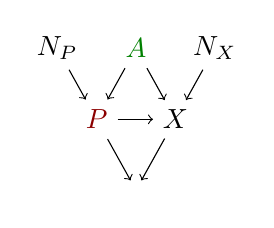
\begin{tikzpicture}
      \pgfmathsetmacro{\dy}{0.9}
      \node (NP) at (-1,0) {$N_P$};
      \node[thick, Green] (A) at (0,0) {$A$};
      \node (NX) at (1,0) {$N_X$};
      \node[thick, DarkRed] (P) at (-0.5,-\dy) {$P$};
      \node (X) at (0.5,-\dy) {$X$};
      \node (R) at (0,-2*\dy) {$\hR$};
      \node[draw=none] at (-0.7,-2*\dy) {$\tcG$};
      \draw[->] (NP) -- (P);
      \draw[->] (A) -- (P);
      \draw[->] (A) -- (X);
      \draw[->] (NX) -- (X);
      \draw[->] (P) -- (X);
      \draw[->] (P) -- (R);
      \draw[->] (X) -- (R);
    \end{tikzpicture}%
    \hspace{0.5cm}
    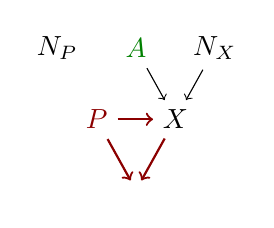
\begin{tikzpicture}
      \pgfmathsetmacro{\dy}{0.9}
      \node (NP) at (-1,0) {$N_P$};
      \node[thick, Green] (A) at (0,0) {$A$};
      \node (NX) at (1,0) {$N_X$};
      \node[thick, DarkRed, double] (P) at (-0.5,-\dy) {$P$};
      \node (X) at (0.5,-\dy) {$X$};
      \node (R) at (0,-2*\dy) {$\hR$};
      \node[draw=none] at (-0.7,-2*\dy) {$\cG$};
      \draw[thick, DarkRed, ->] (P) -- (X);
      \draw[thick, DarkRed, ->] (X) -- (R);
      \draw[thick, DarkRed, ->] (P) -- (R);
      \draw[->] (A) -- (X);
      \draw[->] (NX) -- (X);
    \end{tikzpicture}%
    \caption{A template graph~$\tcG$ for proxy discrimination (left) with its
    intervened version~$\cG$ (right). While from the benevolent viewpoint we do not generically prohibit any
    influence from~$A$ on~$\hR$, we want to guarantee that the proxy~$P$ has no
    overall influence on the prediction, by adjusting~$P \to \hR$ to cancel the
    influence along~$P \to X \to \hR$ in the intervened graph.}
  \label{fig:proxytemplate}
  \end{minipage}%
  \hfill
  \begin{minipage}{0.45\textwidth}
    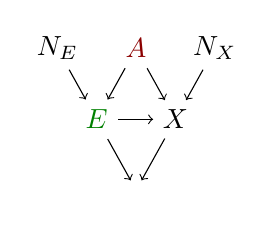
\begin{tikzpicture}
      \pgfmathsetmacro{\dy}{0.9}
      \node (NE) at (-1,0) {$N_E$};
      \node[thick, DarkRed] (A) at (0,0) {$A$};
      \node (NX) at (1,0) {$N_X$};
      \node[thick, Green] (E) at (-0.5,-\dy) {$E$};
      \node (X) at (0.5,-\dy) {$X$};
      \node (R) at (0,-2*\dy) {$\hR$};
      \node[draw=none] at (-0.7,-2*\dy) {$\tcG$};
      \draw[->] (NE) -- (E);
      \draw[->] (A) -- (E);
      \draw[->] (A) -- (X);
      \draw[->] (NX) -- (X);
      \draw[->] (E) -- (X);
      \draw[->] (E) -- (R);
      \draw[->] (X) -- (R);
    \end{tikzpicture}%
    \hspace{0.5cm}
    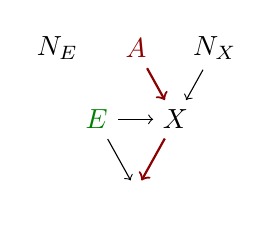
\begin{tikzpicture}
      \pgfmathsetmacro{\dy}{0.9}
      \node (NE) at (-1,0) {$N_E$};
      \node[thick, DarkRed] (A) at (0,0) {$A$};
      \node (NX) at (1,0) {$N_X$};
      \node[thick, Green, double] (E) at (-0.5,-\dy) {$E$};
      \node (X) at (0.5,-\dy) {$X$};
      \node (R) at (0,-2*\dy) {$\hR$};
      \node[draw=none] at (-0.7,-2*\dy) {$\cG$};
      \draw[thick, DarkRed, ->] (A) -- (X);
      \draw[thick, DarkRed, ->] (X) -- (R);
      \draw[->] (NX) -- (X);
      \draw[->] (E) -- (X);
      \draw[->] (E) -- (R);
    \end{tikzpicture}%
    \caption{A template graph~$\tcG$ for unresolved discrimination (left) with
    its intervened version~$\cG$ (right). While from the skeptical viewpoint we generically do not want~$A$
    to influence~$\hR$, we first intervene on~$E$ interrupting all paths
    through~$E$ and only cancel the remaining influence on~$A$ to~$R$.}
    \label{fig:explanatorytemplate}
  \end{minipage}
\end{center}
\end{figure}

% ----------------------------- SUBSECTION  -----------------------------------
\subsection{Avoiding proxy discrimination}
\label{subsec:proxydiscrimination}

While presenting the general procedure, we illustrate each step in the example
shown in \figref{fig:proxytemplate}. A protected attribute~$A$ affects a
proxy~$P$ as well as a feature~$X$. Both~$P$ and~$X$ have additional unobserved
causes~$N_P$ and~$N_X$, where~$N_P, N_X, A$ are pairwise independent. Finally,
the proxy also has an effect on the features~$X$ and the predictor~$\hR$ is
a function of~$P$ and~$X$. Given labeled training data, our task is to find a
good predictor that exhibits no proxy discrimination within a hypothesis class
of functions~$R_{\theta}(P, X)$ parameterized by a real valued vector~$\theta$.

We now work out a formal procedure to solve this task under specific assumptions
and simultaneously illustrate it in a fully linear example, \ie{} the structural
equations are given by
\begin{equation*}
  P = \alpha_P A + N_P, \qquad
  X = \alpha_X A + \beta P + N_X, \qquad
  \hR_{\theta} = \lambda_P P + \lambda_X X \eqp
\end{equation*}
Note that we choose linear functions parameterized by~$\theta = (\lambda_P,
\lambda_X)$ as the hypothesis class for~$R_{\theta}(P, X)$.

We will refer to the \emph{terminal ancestors of a node~$V$ in a causal
graph~$\mathcal{D}$}, denoted by~$ta^{\mathcal{D}}(V)$, which are those
ancestors of~$V$ that are also root nodes of~$\mathcal{D}$. Moreover, in the
procedure we clarify the notion of \emph{expressibility}, which is an assumption
about the relation of the given structural equations and the hypothesis class we
choose for~$R_{\theta}$.

\begin{proposition}\label{pro:proxydisc}
  If there is a choice of parameters~$\theta_0$ such that~$R_{\theta_0}(P,X)$ is
  constant with respect to its first argument and the structural equations are
  \emph{expressible}, the following procedure returns a predictor from the given
  hypothesis class that exhibits no proxy discrimination and is non-trivial in
  the sense that it can make use of features that exhibit potential proxy
  discrimination.
\end{proposition}

\begin{enumerate}
  \item Intervene on~$P$ by removing all incoming arrows and replacing the
    structural equation for~$P$ by~$P=p$. For the example in
    \figref{fig:proxytemplate},
    \begin{equation} \label{eq:proxyR}
      P = p, \qquad
      X = \alpha_X A + \beta P + N_X, \qquad
      \hR_{\theta} = \lambda_P P + \lambda_X X \eqp
    \end{equation}
  \item Iteratively substitute variables in the equation for~$\hR_{\theta}$ from
    their structural equations until only root nodes of the intervened graph are
    left, \ie{} write~$R_{\theta}(P, X)$ as~$R_{\theta}(P, g(ta^{\cG}(X)))$ for
    some function~$g$. In the example,~$ta(X) = \{A, P, N_X\}$ and
    \begin{equation}\label{eq:proxyRroots}
      \hR_{\theta} = (\lambda_P + \lambda_X \beta) p + \lambda_X (\alpha_X A + N_X) \eqp
    \end{equation}
  \item We now require the distribution of~$\hR_{\theta}$
    in~\eqref{eq:proxyRroots} to be independent of~$p$, \ie{} for all~$p, p'$
    \begin{equation}\label{eq:proxyconstraint}
      \bP((\lambda_P + \lambda_X \beta) p  + \lambda_X (\alpha_X A + N_X)) =
      \bP((\lambda_P + \lambda_X \beta) p' + \lambda_X (\alpha_X A + N_X)) \eqp
    \end{equation}
    We seek to write the predictor as a function of~$P$ and all the other roots
    of~$\cG$ separately. If our hypothesis class is such that there
    exists~$\tilde{\theta}$ such that~$R_{\theta}(P, g(ta(X))) =
    R_{\tilde{\theta}}(P, \tilde{g}(ta(X) \setminus \{P\}))$, we call the
    structural equation model and hypothesis class specified
    in~\eqref{eq:proxyR} \emph{expressible}. In our example, this is possible
    with~$\tilde{\theta} = (\lambda_P + \lambda_X \beta, \lambda_X)$
    and~$\tilde{g} = \alpha_X A + N_X$. Equation~\eqref{eq:proxyconstraint} then
    yields the \emph{non-discrimination constraint}~$\tilde{\theta} = \theta_0$.
    Here, a possible~$\theta_0$ is~$\theta_0 = (0, \lambda_X)$, which simply
    yields~$\lambda_P = -\lambda_X \beta$.
  \item Given labeled training data, we can optimize the
    predictor~$\hR_{\theta}$ within the hypothesis class as given in
    \eqref{eq:proxyR}, subject to the non-discrimination constraint. In the
    example
    \begin{equation*}
      \hR_{\theta} = -\lambda_X \beta P + \lambda_X X = \lambda_X (X - \beta P) \eqc
    \end{equation*}
    with the free parameter~$\lambda_X \in \bR$.
\end{enumerate}

In general, the non-discrimination constraint~\eqref{eq:proxyconstraint} is by
construction just~$\bP(R \given do(P=p)) = \bP(R \given do(P=p'))$, coinciding
with Definition~\ref{def:overalldisc}.  Thus Proposition~\ref{pro:proxydisc}
holds by construction of the procedure. The choice of~$\theta_0$ strongly
influences the non-discrimination constraint.  However, as the example shows, it
allows~$R_{\theta}$ to exploit features that exhibit potential proxy
discrimination.

% ----------------------------- SUBSECTION  -----------------------------------
\subsection{Avoiding unresolved discrimination}
\label{subsec:unexplaineddiscrimination}

We proceed analogously to the previous subsection using the example graph in
\figref{fig:explanatorytemplate}. Instead of the proxy, we consider a resolving
variable~$E$. The causal dependences are equivalent to the ones in
\figref{fig:proxytemplate} and we again assume linear structural equations
\begin{equation*}
  E = \alpha_E A + N_E, \qquad
  X = \alpha_X A + \beta E + N_X, \qquad
  \hR_{\theta} = \lambda_E E + \lambda_X X \eqp
\end{equation*}

Let us now try to adjust the previous procedure to the context of avoiding
unresolved discrimination.

\begin{enumerate}
  \item Intervene on~$E$ by fixing it to a random variable~$\eta$
    with~$\bP(\eta) = \bP(E)$, the marginal distribution of~$E$ in~$\tcG$, see
    \figref{fig:explanatorytemplate}. In the example we find
    \begin{align} \label{eq:explanatoryR}
      E = \eta, \qquad
      X = \alpha_X A + \beta E + N_X, \qquad
      \hR_{\theta} = \lambda_E E + \lambda_X X \eqp
    \end{align}
  \item By iterative substitution write $R_{\theta}(E, X)$ as~$R_{\theta}(E,
    g(ta^{\cG}(X)))$ for some function~$g$, \ie{} in the example
    \begin{equation}\label{eq:explanatoryRroots}
      \hR_{\theta} = (\lambda_E + \lambda_X \beta) \eta + \lambda_X \alpha_X A + \lambda_X N_X \eqp
    \end{equation}
  \item We now demand the distribution of~$\hR_{\theta}$
    in~\eqref{eq:explanatoryRroots} be invariant under interventions on~$A$,
    which coincides with conditioning on~$A$ whenever~$A$ is a root of~$\tcG$.
    Hence, in the example, for all~$a, a'$
    \begin{equation}\label{eq:explanatoryconstraint}
      \bP((\lambda_E + \lambda_X \beta) \eta + \lambda_X \alpha_X a + \lambda_X N_X)) =
      \bP((\lambda_E + \lambda_X \beta) \eta + \lambda_X \alpha_X a' + \lambda_X N_X)) \eqp
    \end{equation}
\end{enumerate}

Here, the subtle asymmetry between proxy discrimination and unresolved
discrimination becomes apparent. Because~$R_{\theta}$ is not explicitly a
function of~$A$, we cannot cancel implicit influences of~$A$ through~$X$. There
might still be a~$\theta_0$ such that~$R_{\theta_0}$ indeed
fulfils~\eqref{eq:explanatoryconstraint}, but there is no principled way for us
to construct it. In the example,~\eqref{eq:explanatoryconstraint} suggests the
obvious \emph{non-discrimination constraint}~$\lambda_X = 0$. We can then
proceed as before and, given labeled training data, optimize~$\hR_{\theta} =
\lambda_E E$ by varying~$\lambda_E$. However, by setting~$\lambda_X = 0$, we
also cancel the path~$A \to E \to X \to R$, even though it is blocked by a
resolving variable.  In general, if~$R_{\theta}$ does not have access to~$A$, we
can not adjust for unresolved discrimination without also removing resolved
influences from~$A$ on~$R_{\theta}$.

If, however,~$R_{\theta}$ is a function of~$A$, \ie{} we add the term~$\lambda_A
A$ to~$R_{\theta}$ in~\eqref{eq:explanatoryR}, the non-discrimination constraint
is~$\lambda_A = - \lambda_X \alpha_X$ and we can proceed analogously to the
procedure for proxies.

% ----------------------------- SUBSECTION  -----------------------------------
\subsection{Relating proxy discriminations to other notions of fairness}
\label{sec:variants}

Motivated by the algorithm to avoid proxy discrimination, we discuss some
natural variants of the notion in this section that connect our interventional
approach to individual fairness and other proposed criteria. We consider a
generic graph structure as shown on the left in \figref{fig:generalgraph}. The
proxy~$P$ and the features~$X$ could be multidimensional. The empty circle in
the middle represents any number of variables forming a DAG that respects the
drawn arrows.  \Figref{fig:proxytemplate} is an example thereof. All dashed
arrows are optional depending on the specifics of the situation.

\begin{figure}
  \centering
  \begin{tikzpicture}
  \pgfmathsetmacro{\d}{1.5}
  \pgfmathsetmacro{\dy}{1.2}
    \node[minimum height=1cm] (C) at (0,0) {DAG};
    \node (A) at (-1.5*\d, \dy) {$A$};
    \node (P) at (-0.5*\d, \dy) {$P$};
    \node (R) at ( 0.5*\d, \dy) {$\hR$};
    \node (X) at ( 1.5*\d, \dy) {$X$};
    \draw[->] (A) -- (P);
    \draw[->, dashed] (A) -- (C);
    \draw[<->, dashed] (P) -- (C);
    \draw[<->, dashed] (X) -- (C);
    \draw[->, dashed] (P) -- (R);
    \draw[->] (X) -- (R);
    \node[draw=none] (L) at (-\d,0) {$\tcG$};
  \end{tikzpicture}%
  \hspace{2cm}
  \begin{tikzpicture}
  \pgfmathsetmacro{\d}{1.5}
  \pgfmathsetmacro{\dy}{1.2}
    \node[minimum height=1cm] (C) at (0,0) {DAG};
    \node (A) at (-1.5*\d, \dy) {$A$};
    \node (P) at (-0.5*\d, \dy) {$P$};
    \node (R) at ( 0.5*\d, \dy) {$\hR$};
    \node (X) at ( 1.5*\d, \dy) {$X$};
    \draw[->, dashed] (A) -- (C);
    \draw[->, dashed] (P) -- (C);
    \draw[->, dashed] (P) -- (C);
    \draw[<->, dashed] (X) -- (C);
    \draw[->, dashed] (P) -- (R);
    \draw[->] (X) -- (R);
    \node[draw=none] (L) at (-\d,0) {$\cG$};
  \end{tikzpicture}%
  \caption{{\em Left:} A generic graph~$\tcG$ to describe proxy discrimination.
  {\em Right:} The graph corresponding to an intervention on~$P$. The circle
  labeled ``DAG'' represents any sub-DAG of~$\tcG$ and~$\cG$ containing an
  arbitrary number of variables that is compatible with the shown arrows. Dashed
  arrows can, but do not have to be present in a given scenario.}
\label{fig:generalgraph}
\end{figure}

\begin{definition}\label{def:nondisc}
  A predictor~$\hR$ exhibits no \emph{individual proxy discrimination}, if for
  all~$x$ and all~$p, p'$
  \begin{equation*}
    \bP(\hR \given do(P=p), X=x) = \bP(\hR \given do(P=p'), X=x) \eqp
  \end{equation*}
  A predictor~$\hR$ exhibits no \emph{proxy discrimination in expectation}, if
  for all~$p, p'$
  \begin{equation*}
    \E[\hR \given do(P=p)] = \E[\hR \given do(P=p')] \eqp \label{eq:inexp}
  \end{equation*}
\end{definition}

Individual proxy discrimination aims at comparing examples with the same
features~$X$, for different values of~$P$. Note that this can be individuals
with different values for the unobserved non-feature variables. A true
individual-level comparison of the form ``What would have happened to me, if I
had always belonged to another group'' is captured by \emph{counterfactuals} and
discussed in~\cite{Kusner2017, Nabi2017}.

For an analysis of proxy discrimination, we need the structural equations
for~$P, X, \hR$ in \figref{fig:generalgraph}
\begin{subequations}
  \begin{align*}
    P &= \hat{f}_P (pa(P)) \eqc \\
    X &= \hat{f}_X (pa(X)) = f_X (P, ta^{\cG} (X) \setminus \{P\}) \eqc \\
    \hR &= \hat{f}_{\hR} (P, X) = f_{\hR} (P, ta^{\cG} (\hR) \setminus \{P\}) \eqp
  \end{align*}
\end{subequations}
For convenience, we will use the notation~$ta^{\cG}_{P}(X) := ta^{\cG} (X)
\setminus \{P\}$. We can find~$f_X, f_R$ from~$\hat{f}_X, \hat{f}_R$ by first
rewriting the functions in terms of root nodes of the \emph{intervened graph},
shown on the right side of \figref{fig:generalgraph}, and then assigning the
\emph{overall} dependence on $P$ to the first argument.

We now compare proxy discrimination to other existing notions.

\begin{theorem}\label{thm:rvtodistr}
  Let the influence of~$P$ on~$X$ be additive and linear, \ie{}
  \begin{equation*}
    X = f_X (P, ta^{\cG}_P(X)) = g_X(ta^{\cG}_P(X)) + \mu_X P
  \end{equation*}
  for some function~$g_X$ and~$\mu_X \in \bR$. Then any predictor of the form
  \begin{equation*}
    \hR = r(X - \E [X \given do(P)])
  \end{equation*}
  for some function~$r$ exhibits no proxy discrimination.
\end{theorem}

Note that in general~$\E[X \given do(P)] \neq \E[X \given P]$. Since in practice
we only have observational data from~$\tcG$, one cannot simply build a
predictor based on the ``regressed out features''~$\tilde{X} := X - \E[X \given
P]$ to avoid proxy discrimination. In the scenario of
\figref{fig:proxytemplate}, the direct effect of~$P$ on~$X$ along the arrow~$P
\to X$ in the left graph cannot be estimated by~$\E[X \given P]$, because of
the common confounder~$A$. The desired interventional expectation~$\E[X \given
do(P)]$ coincides with~$\E[X \given P]$ only if one of the arrows~$A \to P$
or~$A \to X$ is not present. Estimating direct causal effects is a hard problem,
well studied by the causality community and often involves instrumental
variables~\cite{Angrist2001}.

This cautions against the natural idea of using~$\tilde{X}$ as a ``fair
representation'' of~$X$, as it implicitly neglects that we often want to remove
the effect of proxies and not the protected attribute. Nevertheless, the notion
agrees with our interventional proxy discrimination in some cases.

\begin{corollary}\label{cor:rvtodistr}
  Under the assumptions of Theorem~\ref{thm:rvtodistr}, if all directed paths
  from any ancestor of~$P$ to~$X$ in the graph~$\cG$ are blocked by~$P$, then
  any predictor based on the \emph{adjusted features}~$\tilde{X} := X - \E[X
  \given P]$ exhibits no proxy discrimination and can be learned from the
  observational distribution~$\bP(P, X, Y)$ when target labels~$Y$ are
  available.
\end{corollary}

Our definition of proxy discrimination in expectation (\ref{eq:inexp}) is
motivated by a weaker notion proposed in~\cite{Calders2010}. It asks for the
expected outcome to be the same across the different populations~$\E[R \given
P=p] = \E[R \given P=p'].$ Again, when talking about proxies, we must be careful
to distinguish conditional and interventional expectations, which is captured by
the following proposition and its corollary.

\begin{proposition}\label{pro:inexpectation}
  Any predictor of the form~$\hR = \lambda (X - \E[X \given do(P)]) + c$
  for~$\lambda, c \in \bR$ exhibits no proxy discrimination in expectation.
\end{proposition}

From this and the proof of Corollary~\ref{cor:rvtodistr} we conclude the
following Corollary.

\begin{corollary}
  If all directed paths from any ancestor of~$P$ to~$X$ are blocked by~$P$, any
  predictor of the form~$\hR = r(X - \E[X \given P])$ for linear~$r$ exhibits no
  proxy discrimination in expectation and can be learned from the observational
  distribution~$\bP(P, X, Y)$ when target labels~$Y$ are available.
\end{corollary}
